\documentclass{article}
\usepackage{amsmath,amssymb}
\usepackage[margin=3cm]{geometry}
\usepackage{graphicx}
\usepackage{syntax}
\usepackage{dirtree}
\usepackage{longtable}
\usepackage{pgfplots}
\usepackage{hyperref}

\setlength{\parindent}{0pt}
\setlength{\parskip}{0.7em}

\begin{document}

\title{\texttt{randexam}: Randomized Exam Generation and Grading\\[1em] User Manual\\[1em] \Large Version 1.11.0}
\date{\vspace*{-2em}2015-01-29}
\maketitle

\section{Overview}

The \texttt{randexam} program allows the generation of
individually-randomized exams for every student. The process starts
with a \emph{library} latex file that contains a sequence of
\emph{zones}. Each zone contains a sequence of \emph{questions}, and
each question contains one or more \emph{variants}. If the question is
a multiple-choice question, then each variant has a set of
\emph{answers}, exactly one of which is the \emph{correct answer}.

Each randomized exam has the same set of zones as the library, and in
the same order. Within each zone, the order of questions is
randomized. For each question, one of the variants is selected at
random, and the order of the answers is also randomized.

There are two important identifiers used by \texttt{randexam}: the
\emph{NetID} identifies students and the \emph{exam key} identifies
exams. The exam key is a string of the form \texttt{BAECCD}, where the
number of letters depends on the number of randomized exams
generated. The exam key uniquely identifies the randomized exam, and
so it is written on the front of the exam booklet and must be copied
by the student onto the Scantron sheet, where it is encoded into the
last few questions on the Scantron.

The exam keys for a particular exam are generated so that they all
differ by at least three letters. This means that if a student makes
an error in copying their exam key, they won't accidentally produce
another valid exam key. In particular, if they make only a
single-letter error, then it is possible to correct this
automatically, and mis-copying two letters can be detected but not
automatically corrected. If they mis-copy three or more letters,
however, then they may produce another valid key, and this can only be
detected by observing that their score was very low (effectively
random guessing). In practice this has never occurred.

\section{Preparing the exams}

\begin{enumerate}
\item Obtain a copy of the three files: \texttt{randexam},
  \texttt{config.ini}, and \texttt{library.tex}.
\item On Mac or Linux, make sure \texttt{randexam} is executable, or
  make it so with \texttt{chmod +x randexam}.
\item On Windows, it may be necessary to rename \texttt{randexam} to
  \texttt{randexam.py} and to run it with \texttt{python randexam.py
    <arguments>} rather than \texttt{./randexam <arguments>}.
\item Set the \texttt{exam_title} in \texttt{config.ini}.
\item Set the \texttt{filename_prefix} in \texttt{config.ini} to
  \texttt{TAM212_F14_Midterm2} or similar, and correspondingly rename
  \texttt{library.tex} to
  \texttt{TAM212_F14_Midterm2_library.tex}. Hereafter we write
  \texttt{XXX} in place of the prefix, so this file is referred to as
  \texttt{XXX_library.tex}.
\item Edit \texttt{XXX_library.tex} to add questions and make the
  cover sheet. This file can be latexed to produce the library PDF
  file that contains all variants of all questions.
\item Run \texttt{./randexam proc-lib}. This will produce the output
  tex file as well as various files summarizing the randomization,
  question points, and so on.
\item Run \texttt{pdflatex XXX_exams.tex}, and look at the output near
  the end for information about exam lengths.
\item To ensure all exams have the same number of pages and the last
  page is blank, adjust \texttt{minimum_pages_per_exam} in
  \texttt{randexam} to be the smallest even number that is at least $N
  + 1$, where $N$ is the maximum raw length reported by latex when
  processing \texttt{XXX_exams.tex}. Then re-run \texttt{./randexam
    proc-lib} and re-latex.
\end{enumerate}

\begin{figure}
  \centering
  \includegraphics{pipeline}
  \caption{The pipeline for making and grading the randomized
    exams. The green pentagons are input files that require human
    effort to generate, the purple boxes are output files, the yellow
    ellipses are program runs, and the pink hexagon is the students
    sitting the exam and the scanning of the Scantron forms.}
  \label{fig:pipeline}
\end{figure}

\section{Tips for exam preparation}

\begin{enumerate}
\item Try to have about three variants of each question. The variants
  should be of equal difficulty and should only differ in some
  unimportant way. For example, reverse the orientation of a figure,
  change the value of one number, etc.
\item Zones serve two purposes: (1) to group questions so that random
  permutations only occur within a zone, not between zones (allowing
  the exam to start with 5 easy questions, for example); and (2) to
  insert text at a certain point in the exam. Zones do not need to
  contain any questions, so they can be used just to insert text, for
  example a formula sheet at the start or end of the exam.
\item Points are assigned on a per-question basis, so all variants of
  a given question are worth the same number of points.
\item Only one answer can be marked as correct for each variant. This
  answer will be awarded the full points for that question, and all
  other answers will be worth zero points. This can be adjusted by
  manually editing \texttt{XXX_points.csv}, which allows points to be
  assigned to any answer of any variant in an arbitrary way, including
  negative points and real-valued points.
\item Questions do not have any text associated with them directly. If
  there is text that is common to all variants of a question then it
  must be repeated in each variant.
\item Variants are not required to have any answers. This is useful
  for including questions that the students must answer via some other
  means, such as a long-form written answer.
\item Using PGFPlots for graphics (based on PGF/TikZ) can result in
  very long compile times and errors like \texttt{TeX capacity
    exceeded, sorry}. To avoid this, use the PGFPlots
  \texttt{external} library. To do this:
  \begin{enumerate}
  \item Include the following lines in the library file preamble:
\begin{verbatim}
\usepgfplotslibrary{external}
\tikzexternalize
\end{verbatim}
  \item Use \verb+\tikzsetnextfilename+ to assign a unique filename for
    each \texttt{tikzpicture}, such as:
\begin{verbatim}
\tikzsetnextfilename{tikz_figname}
\begin{tikzpicture}
...
\end{tikzpicture}
\end{verbatim}
  \item Generate library and exam PDFs with:
\begin{verbatim}
pdflatex -shell-escape filename.tex
\end{verbatim}
  \item To generate student feedback, all the TikZ files must be in
    the current directory, so copy them over if they are somewhere
    else. This is both because latex isn't being run with
    \texttt{-shell-escape} when generating feedback, and because the
    use of \texttt{-output-directory} is incompatible with the TikZ
    external file support.
  \end{enumerate}
\end{enumerate}

\section{Configuration Options}

\hangindent=1cm \texttt{answers_per_question} (default: \texttt{5})
Number of possible answers per question on the Scantron form. That is,
the number of Scantron bubbles for each question.

\hangindent=1cm \texttt{check_repeated_exam_keys} (default:
\texttt{Yes}) Check for repeated use of each exam key, and report when
this happens. If you are using individualized exams then this should
not occur.

\hangindent=1cm \texttt{check_valid_netids} (default: \texttt{Yes})
Check whether all students taking the exam have NetIDs listed in the
\texttt{XXX_netids.txt} file.

\hangindent=1cm \texttt{curve_scores} (default: \texttt{No}) Whether
to transform the final exam scores by a curving function.

\hangindent=1cm \texttt{curve_new_median} (default: \texttt{80}) If
curving is enabled, then this is the new median score of the curved
scores.

\hangindent=1cm \texttt{curve_new_zero} (default: \texttt{20}) If
curving is enabled, then this is the new curved score than an uncurved
value of zero will map to.

\hangindent=1cm \texttt{exam_title} (default: \texttt{Exam}) Title of
the exam (used in statistics reports).

\hangindent=1cm \texttt{feedback_directory} (default:
\texttt{feedback}) Directory name where feedback PDFs are stored.

\hangindent=1cm \texttt{feedback_solutions} (default: \texttt{Yes})
Whether per-student feedback should include full solutions to all
questions.

\hangindent=1cm \texttt{filename_prefix} (default: \emph{blank})
Prefix to append to all input and output filenames. This is the
\texttt{XXX} in filenames like \texttt{XXX_library.tex}.  The
filename_prefix should uniquely specify the exam. For example,
\texttt{TAM212_S13_Final} would indicate the final exam in Spring 2013
for the course TAM 212.

\hangindent=1cm \texttt{last_scantron_question_number} (default:
\texttt{96}) Number of the last question on the Scantron form. This is
used to determine the questions that will store the exam key.

\hangindent=1cm \texttt{mail_domain} (default: \texttt{illinois.edu})
Domain name to append to student NetID to produce email addresses.

\hangindent=1cm \texttt{mail_max_attempts} (default: \texttt{5})
Maximum number of times to retry sending each feedback email before
giving up.

\hangindent=1cm \texttt{mail_max_per_second} (default: \texttt{1})
Maximum email sending rate, in emails per second.

\hangindent=1cm \texttt{mail_message_text} (default: \texttt{The
  attached file contains your test results.}) Text to use in the
feedback email.

\hangindent=1cm \texttt{mail_retry_delay_seconds} (default:
\texttt{30}) Number of seconds to delay between retries of failed
feedback email sending.

\hangindent=1cm \texttt{mail_server} (default:
\texttt{smtp.illinois.edu}) SMTP mail server to use for outgoing
feedback emails.  Connections will be made on port 587 using TLS and
authenticated with the provided username/password.

\hangindent=1cm \texttt{mail_signature_file} (default:
\texttt{$\sim$/.signature}) Signature file to include at the end of
feedback email messages, if the file exists.

\hangindent=1cm \texttt{mail_timeout_seconds} (default: \texttt{120})
Timeout for all mail operations (connecting, sending, etc).
Operations that take longer than this will be considered an error.

\hangindent=1cm \texttt{max_answers_per_question} (default:
\texttt{3}) Maximum number of answers for a question to still receive
some partial credit. Only used if
\texttt{multiple_answers_per_question} is \texttt{Yes}.

\hangindent=1cm \texttt{minimum_pages_per_exam} (default: \texttt{2})
Length that every exam will be padded out to. Should be the smallest
even number at least equal to $N + 1$, where $N$ is the maximum raw
length reported by latex when processing \texttt{XXX_exams.tex}.

\hangindent=1cm \texttt{multiple_answers_per_question} (default:
\texttt{No}) Whether multiple answers per question are permitted (if
more than one answer is given, then partial credit is awarded in
inverse proportion to the number of given answers).

\hangindent=1cm \texttt{number_of_exams} (default: \texttt{1}) Number
of randomized exam papers to generate.

\hangindent=1cm \texttt{one_page_per_question} (default: \texttt{No})
Whether the randomized exams should be formatted with every question
on a different page.

\hangindent=1cm \texttt{random_seed} (default: \texttt{7}) Seed value
for the random number generator that creates the randomized
exams. Random numbers are only generated during \texttt{randexam
  proc-lib}. The same value of random_seed will result in the same
randomized exam generation, assuming the same version of Python on the
same computer.

\hangindent=1cm \texttt{randomize_answers} (default: \texttt{Yes}) If
\texttt{Yes} then choose answer order randomly, otherwise leave
answers in the library order.

\hangindent=1cm \texttt{randomize_questions} (default: \texttt{Yes})
If \texttt{Yes}, then choose the question order randomly within zones,
otherwise leave questions in the library order.

\hangindent=1cm \texttt{randomize_variants} (default: \texttt{Yes}) If
\texttt{Yes}, then choose question variants randomly. If \texttt{No},
then choose question variants in order, so exam 1 has variant 1 of
each question, exam 2 has variant 2 of each question, etc. After
exhausting all variants of a question, the selection will cycle back
to variant 1.

\hangindent=1cm \texttt{raw_scan_directory} (default: \emph{blank})
Directory name where image scans of the Scantrons forms are stored. If
blank, then these are ignored. If non-blank, these scans are attached
to feedback emails.

\hangindent=1cm \texttt{score_decimals} (default: 1)
The number of decimal places to which total scores are truncated.

\section{Administering the exams}

\begin{enumerate}
\item Send the \texttt{XXX_exams.pdf} file
  containing all the exams to Document Services, via a department
  secretary. The instructions should be something like:

  \rule{\linewidth}{0.5pt}

  \parbox{\linewidth}{
    \tt
    Printing type: double-sided, staple every 11 sheets of paper (that is, every 22 PDF pages) to form 700 total exam papers \\
    Deliver to: MEB 160 by Thursday morning (Oct 16)
  }

  \rule{\linewidth}{0.5pt}

  Here the number 22 is the value of \texttt{minimum_pages_per_exam} and
  11 is half of this value. In the case the PDF file should have $22
  \times 700 = 15\,400$ total PDF pages.
\item Obtain Scantron sheets from CITL Exam Services (Armory
  247). These are free.
\item Hand out the exam booklets and Scantron sheets to
  students. Instruct them to fill in their information on the Scantron
  sheet and on the exam booklet. They should pay special attention to
  completing their NetID on the Scantron and correctly encoding the
  exam key from the exam booklet onto the last few questions on the
  Scantron.
\item Have the students do the exam.
\item Collect both the Scantron sheets and the exam papers (with names
  on them) from the students, so that exam papers can be later matched
  to students if needed. Ensure that the NetID and Exam Key (the last
  few questions on the Scantron) are filled in for every student.
\item Arrange the Scantron forms so that the cut corners are all
  aligned.
\item Take the Scantrons to CITL Exam Services (Armory 247). Tell them
  that you want the ``dot dat'' file sent to you. This refers to a
  filename like \texttt{jd17699.dat} that contains the raw scantron
  data.
\end{enumerate}

\section{DRES students}

\begin{enumerate}
\item Inform DRES students before the exam that they should schedule
  their exams at the DRES facility. Tell DRES that the allowed window
  for the exam is from the afternoon on the day of the exam to the
  evening of the day following.
\item Extract individual exam PDFs from the large
  \texttt{XXX_exams.pdf} file and call these \texttt{DRES1.pdf},
  \texttt{DRES2.pdf}, etc. This can be done using Adobe Acrobat Pro,
  or on Mac OS X using Preview and Print to PDF.
\item Email these individual PDFs to DRES and tell DRES that the
  students need to use an orange 96-question Scantron form, and that
  you want both the exam paper and the Scantron form returned to you.
\end{enumerate}

\section{Conflict exams}

\begin{enumerate}
\item Schedule conflict exams starting 2 hours before the real exam
  (assuming a 2-h exam) until the afternoon of the following day. A
  good timeslot is 7~am the morning after the real exam, which ensures
  that only students who really need the conflict will use it.
\item Conflict exams can use the same exam as the real exam, as we
  rely on the randomization to make cheating difficult.
\item Conflict exams should be administered using printed copies of
  the exam from the main printing.
\end{enumerate}

\section{Grading the exams}

\begin{enumerate}
\item Obtain the \texttt{jdXXXX.dat} file from Exam Services and
  rename it to \texttt{XXX_scantron.dat} or similar.
\item Extra exams, such as DRES or conflicts, can be hand-entered into
  the \texttt{scantron.dat} file. The format of lines in this file is
  described in detail in \texttt{randexam-dev-manual.pdf}.
\item By default, \texttt{randexam} will look for a file called
  \texttt{XXX_netids.txt} in the current directory. This should
  contain the class roster, listed as one NetID per line, and is used
  to check validity of the NetIDs in \texttt{scantron.dat}. If this
  checking is not desired then set \texttt{check_valid_netids: No}
  in \texttt{randexam}.
\item Run \texttt{./randexam proc-scan} and clean up errors in the
  \texttt{scantron.dat} file as needed. It is essential that every
  student has a correct exam key for grading to occur, and their NetID
  should also be correct for email sending and gradebook
  uploads. Other data (name, student ID, etc) is only for
  informational and checking purposes.
\item If desired, hand-edit the \texttt{XXX_points.csv} file to change the
  number of points awarded for each variant of each question. This is
  a good way to give all students full points for a given question, if
  a question was badly worded or incorrect.
\item Run \texttt{./randexam proc-ans} to perform the actual
  grading. This will generate exam statistics in tex file and the
  final scores in the files \texttt{XXX_scores.csv} and
  \texttt{XXX_gradebook.csv} (two different formats of the same
  information).
\item Run \texttt{pdflatex XXX_stats.tex} to generate a PDF of the
  exam statistics.
\end{enumerate}

\section{Curving exam scores}

If score curving is enabled (by the \texttt{curve_scores}
configuration parameter) then the final student scores are transformed
using the piecewise linear function shown in Figure~\ref{fig:curve}
with the following parameters:
\begin{center}
  \begin{tabular}{cll}
    quantity & config option & description \\
    \hline
    $M_0$ & --- & median of old (uncurved) scores \\
    $M_1$ & \texttt{curve_new_median} & desired median of new (curved) scores \\
    $Z_1$ & \texttt{curve_new_zero} & desired new (curved) score for old zero score
  \end{tabular}
\end{center}

\begin{figure}
  \centering
  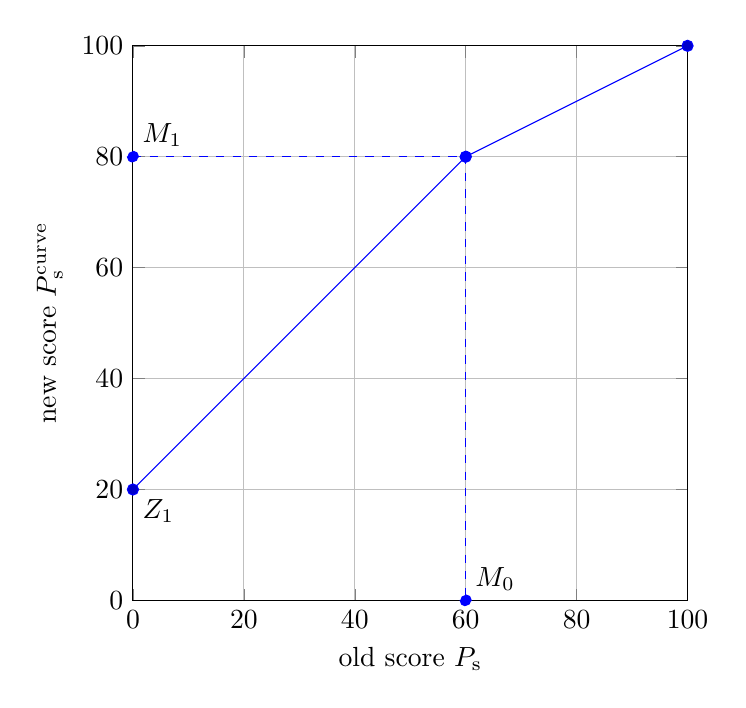
\begin{tikzpicture}
    \begin{axis}[
      width=10cm,
      xlabel={old score $P_{\rm s}$},
      ylabel={new score $P^{\rm curve}_{\rm s}$},
      grid=both,
      axis equal image,
      xmin=0,
      xmax=100,
      ymin=0,
      ymax=100,
      ]
      \node[above right] at (axis cs:60,0) {$M_0$};
      \node[above right] at (axis cs:0,80) {$M_1$};
      \node[below right] at (axis cs:0,20) {$Z_1$};
      \addplot coordinates {
        (0,20)
        (60,80)
        (100,100)
      };
      \addplot[dashed,blue,mark=*] coordinates {
        (0,80)
        (60,80)
        (60,0)
      };
    \end{axis}
  \end{tikzpicture}
  \caption{Curving function that transforms old scores to new scores.}
  \label{fig:curve}
\end{figure}

\section{Allowing partial credit for multiple answers}

\begin{enumerate}
\item If desired, \texttt{randexam} can allow students to fill in
  multiple answers for a single question, and then give partial credit
  for that question if one of the provided answers was correct. To
  achieve this, several changes need to be made to the exam process,
  as follows.
\item When processing the Scantrons at CITL Exam Services, they need
  to scan the exam in a ``multiple answer'' format. This alters the
  \texttt{.dat} file format that they return.
\item Before running \texttt{./randexam proc-scan}, edit
  \texttt{config.ini} and set \texttt{multiple_answers_per_question:
    Yes}.
\item If multiple answers are given for a question, then the student
  is given partial credit if one of them is correct. The amount of
  credit given is inversely proportional to the number of answers they
  gave, so half credit for two answers, one-third credit for three
  answers, etc. In all cases, if the correct answer was not one of the
  given answers then no points are given. The maximum number of
  answers for which partial credit will be awarded is controlled by
  the \texttt{max_answers_per_question} variable.
\end{enumerate}

\section{Interpreting the exam statistics}

\begin{enumerate}
\item The \texttt{XXX_stats.pdf} file contains summary statistics for
  the exam and questions.
\item Check that the median score is reasonable (typically around 80
  to have half the class in the A/B range), and curve the scores if
  desired.
\item Check that all question have variants that are fairly similar to
  each other in relative points. If $R_{\rm QV}$ is less that about
  80\% or more than about 120\%, then investigate why some variants
  are significantly different and consider awarding all students full
  points for that question.
\item Check that all questions have discrimination values of at least
  20\% (higher is better). Very easy questions (difficulty below 10\%)
  can legitimately have low discrimination without this being a
  problem. If a question has difficulty over 10\% and discrimination
  below 20\%, however, then investigate to see whether the question is
  poorly worded or incorrect, and consider awarding all students full
  points for that question.
\end{enumerate}

\section{Uploading scores to Compass}

\begin{enumerate}
\item Go to \texttt{Grade Center $\to$ Full Grade Center} in the
  left-hand menu.
\item Back up the current data with \texttt{Work Offline $\to$
    Download}.
\item Edit the \texttt{XXX_gradebook.csv} file generated by
  \texttt{randexam} to add a new first line consisting of:
  \begin{center}
    \texttt{"Username","Test Name"}
  \end{center}
  where \texttt{Test Name} is replaced by something like
  \texttt{Midterm 2} or \texttt{Final}.
\item Go to \texttt{Work Offline $\to$ Upload} and upload the edited
  \texttt{XXX_gradebook.csv} file.
\item In the grade center, set \texttt{Sort Columns By: Date Created}
  and \texttt{Order: Ascending}.
\item Select \texttt{Edit Column Information} from the drop-down menu
  next to the newly-uploaded column.
\item Set:
  \begin{itemize}
  \item \texttt{Primary Display: Score}
  \item \texttt{Category: Test}
  \item \texttt{Points Possible: 100}
  \item \texttt{Show Statistics: Yes}
  \end{itemize}
\end{enumerate}

\section{Sending feedback emails to students}

\begin{enumerate}
\item Run \texttt{./randexam proc-feedback} to generate per-student
  feedback PDFs. These are created in the directory named by the
  \texttt{feedback_directory} variable in \texttt{config.ini} (by
  default, a \texttt{feedback/} subdirectory). If there are extra
  files needed to latex the feedback, such as figures, then they need
  to be copied by hand into the feedback directory before running
  \texttt{./randexam proc-feedback}.
\item If desired, create a \verb+rawscan+ directory with PDFs of
  individual Scantron sheets to be included in email feedback and
  correspondingly set the \texttt{raw_scan_directory} variable in
  \texttt{config.ini}.
\item Run \texttt{./randexam proc-email}. This will ask for the NetID
  and password of the account that is sending the email.

  To be able to send email directly through the UIUC email servers,
  your NetID needs to be authorized by CITES. This only needs to be
  done once, as it will stay authorized. To do this, send email to the
  CITES Help Desk at \texttt{consult@illinois.edu} with the message
  ``I request IMAP access for my email.''

  After each email has been send, a file is created in the feedback
  directory called \texttt{<NetID>.email_sent}. If \texttt{./randexam
    proc-email} is re-run, then students with such a file won't be
  sent further email. Thus email sending can be retried repeatedly
  until all emails are successfully sent. Deleting the
  \texttt{*.email_sent} files will re-enable sending to those students.
\end{enumerate}

\end{document}
